 \documentclass{beamer}
\usetheme{Berkeley}
%\definecolor{mycolor}{rgb}{.125,0.5,0.25}
%\usecolortheme[named=mycolor]{structure}
% remove the navigation bar
\beamertemplatenavigationsymbolsempty
% set the numbering to fraction 1/n
\setbeamertemplate{frame numbering}[fraction]
% add the frame count to the footer 
\setbeamertemplate{footline}[frame number]
\DeclareMathOperator*{\argmin}{arg\,min}
\usepackage{amsmath}
\usepackage{media9}
\usepackage{hyperref}
\usepackage[options ]{algorithm2e}

\title[Poisson Deblurring]{Poisson Image Deblurring}
\author{Deepan Das, Sek Cheong} 
\institute{University of Wisconsin, Madison}
\date{March 13 2019}

\begin{document}

\begin{frame}
\titlepage
\end{frame}

\section{Introduction}
\begin{frame}[t]{Image Degradation}

The Image Noise Model is one of the most important image degradation models, apart from motion blur and defocus. 

\vspace{1.2cm}

\textbf{Poisson Noise: }This unavoidable noise is caused by the quantum nature of light.

\vspace{0.2cm}
\textbf{Blur: }This is caused by the natural extent of the point spread function of the imaging device.

\vspace{1.2cm}
\textbf{Goal: } Restore a high quality image from blurred images corrupted by Poisson Noise.

\end{frame}

\begin{frame}{Poisson Noise Model}
The various sources of light generally have random fluctuation of photons leading to spatial and temporal randomness. Mathematically, it can be represented as: 

\[
    P(f_{(pi)}=k) = \frac{\lambda^{k}_{i} e^{-\lambda}}{k!}
\] 
\begin{figure}
    \centering
    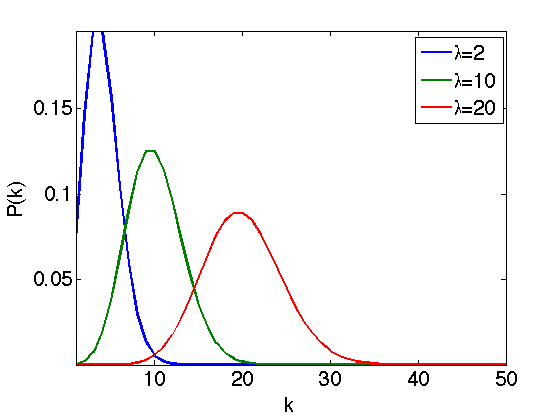
\includegraphics[scale=0.2]{poisson_dist.png}
    \caption{Poisson Distribution}
    \label{fig:my_label}
\end{figure}
\end{frame}


\begin{frame}{Poisson Noise Model}
\begin{figure}[!tbp]
  \centering
  \begin{minipage}[b]{0.45\textwidth}
    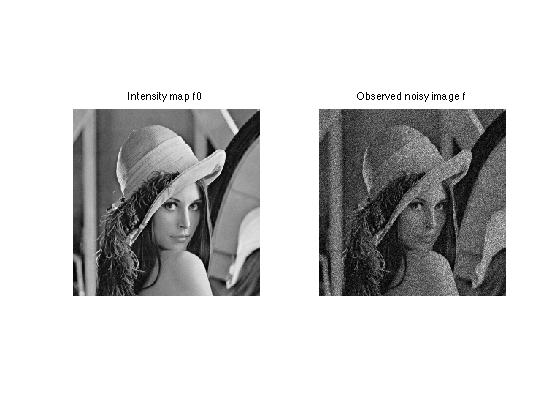
\includegraphics[width=\textwidth]{poisson_img.png}
    \caption{Poisson Image addition}
  \end{minipage}
  \hfill
  \begin{minipage}[b]{0.45\textwidth}
    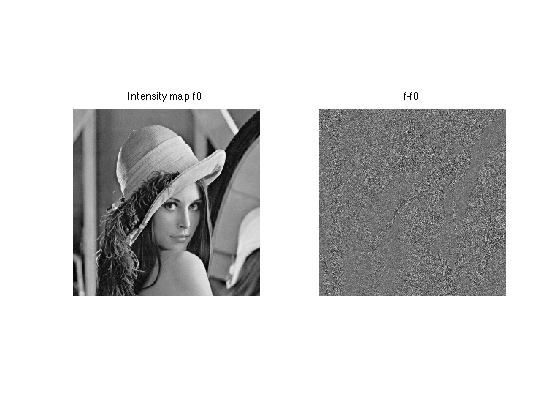
\includegraphics[width=\textwidth]{poisson_diff.png}
    \caption{Difference}
  \end{minipage}
\end{figure}
\end{frame}

\begin{frame}{Degraded Image}
A degraded image can be expressed as:
\[
    f = P(Hu)
\]

\vspace{0.5cm}

\textbf{Challenge: }Linear operator $H$ is usually ill-conditioned. Therefore, deblurring is an ill-posed inverse problem.

\vspace{0.5cm}

\textbf{Previous methods: } Mainly use regularization methods to restrict solution space. Some methods used previously:
\begin{itemize}
    \item Total Variation(TV) : Preserves edges well
    \item Wavelets and Frames: Multi-scale and sparse representation
    \item Hybrid methods
\end{itemize}

\end{frame}

\begin{frame}{Motivation for Patch Priors}
\begin{itemize}
    \item TV generally oversmooths textured images
    \item Wavelet based methods usually involved fixed dictionaries
    \item \textbf{Patch based priors} generally capture the distinctive characteristics of the processed image
    \item \textbf{K-SVD} based approaches learn an optimal over-complete dictionary and then recover each image patch using a linear combination of only a few atoms
\end{itemize}

\textbf{Note: }Poisson noise is signal dependent and Gaussian based models may not be suitable.
\end{frame}

\begin{frame}{Poisson Noise removal}{Motivation}

Assumption: Values of observed image at locations ${i}$ are independent.
\[
P(f|Hu) = \prod_{i}{}\frac{e^{-(Hu)}_i   ((Hu)_i)^{f_i}}{f_i !}
\]
Some of the methods are:
\begin{itemize}
    \item Recover image simply using methods designed for Gaussian removal
    \item Transform Poisson noise to near Gaussian using an appropriate transform (\textbf{Variance Stabilizing Transform})
    \item Remove Poisson noise directly via a data fidelity term derived from Poisson noise statistics
\end{itemize}
    
\end{frame}


\begin{frame}{Data Fidelity Approach}{Bayesian Overview}

Traditional Sparse representation problems were solved using:
\[
    min \frac{1}{2} ||D\alpha - y ||_2^2 + ||\alpha||^p_p
\]

While attempting to remove the Poisson noise, a Bayesian approach like the previous one uses a Total Variation term and a fidelity term
\[
    min ||\nabla u||_1 + \lambda\langle Hu-f\hspace{0.25pt}log Hu,1\rangle
\]
Various methods were proposed to solve this non quadratic function. 
    
\end{frame}

\begin{frame}{Total Variation}{An Introduction}

\textbf{Principle: } Signals with excessive and possibly spurious detail have high total variation.

%\textbf{Use: }Reducing the total variation of the signal subject to it being a close match to the original signal, removes unwanted detail whilst preserving important details such as edges. 

\[
V(x) = \sum_{i,j}{} \sqrt{|x_{i+1,j} - x_{i,j}|^2 + |x_{i,j+1} - x_{i,j}|^2}
\]
The denoising problem still remains the same, but with a modified regularization term dependent on the TV present.
\[
\min_{y} \hspace{0.2cm} E(x,y) + \lambda V(x)
\]


\end{frame}

\begin{frame}{K-SVD for Gaussian Noise}{Quick Recap}

The fundamental assumption of the K-SVD approach is that image patches admit a sparse representation. For Gaussian noise, we have:
\[\min \sum_{(i,j) \in \mathcal{A}_n}{} \mu_{ij}||\alpha_{ij}||_0 + \sum_{(i,j) \in \mathcal{A}_n}{} ||D\alpha_{ij} - R_{ij}u||^2_2  + \lambda ||u-g||^2_2\]

It was also show that learning the dictionary from noise image leads to better performance. 
\end{frame}

\begin{frame}{K-SVD for Gaussian Noise}{Quick Recap}{\textbf{Optimization Steps}}

Elad et al. minimized the expression with respect to $D, \alpha_{ij}$ and $u$ separately
\begin{itemize}
    \item Solve for $D$ given ${\alpha_{ij}}$. Update is done one atom at a time
    \item Use OMP to get an efficient solution for ${\alpha_{ij}}$
    \item Solve for $u$ given $D$ and $\alpha_{i,j}$
\end{itemize}

The K-SVD algorithm provides very good results for Gaussian noise removal and has been generalised for other applications like inpainting, demosaicking, etc.
    
\end{frame}

\section{Proposed Approach}

\begin{frame}{Proposed Model}{Background}
In general denosing a image can be modeled by solving the minimization of loss function:
\[
    L(x) = \frac{1}{2}||x-y||^2 + G(x) 
\]

Where $y$ is a observed image, and $x$ is the unknown ideal image to be recovered \[
\frac{1}{2}||x-y||^2 \quad \textrm{measure of similarity (sanity check)}
\]
\[
G(x) \quad \textrm{is the prior or regularization}
\]
The goal is to come up with a \textbf{good} prior to model the image and its noise distribution. In Bayesian view this is the equivalent of Maximum-A-Posteriori \textbf{MAP} estimation
\end{frame}


\begin{frame}{Proposed Model}{Background}
\begin{itemize}
    \item Suppose we are given a image 
    \[ y=Hx+v \]
    Which is nosiy and degraded version of $x$
    \item How do we go about solving $x$?
\end{itemize}
\end{frame}


\begin{frame}{Proposed Model}{Background}
\begin{itemize}
    \item Suppose we are given a image 
    \[ y=Hx+v \]
    Which is nosiy and degraded version of $x$
    \item How do we go about solving $x$?
    \item Assume $x$ from $D\alpha$
\end{itemize}
\end{frame}

\begin{frame}{Proposed Model}{Background}
\begin{itemize}
    \item Suppose we are given a image 
    \[ y=Hx+v \]
    Which is nosiy and degraded version of $x$
    \item How do we go about solving $x$?
    \item Assume $x$ from $D\alpha$
    \item How about find the $\alpha$ that generated $y$?
\end{itemize}
\end{frame}

\begin{frame}{Proposed Model}{Background}
With sparse model, given a noisy image $y=Hx+v$ \footnote{in inprinting problem $H$ is a lost sample $W$ the   $\hat{\alpha} = \argmin_{\alpha}||\alpha||_0 \quad
    \textrm{s.t.} \quad
    ||y-WD\alpha||\le \epsilon$ } we can denoise it by solving:
\[
    \hat{\alpha} = \argmin_{\alpha}||\alpha||_0 \quad
    \textrm{s.t.} \quad
    ||y-D\alpha||\le \epsilon
\]

\[
    \hat{x} = D\hat{\alpha} 
\]
Why does it work?
\[
    ||\hat{\alpha}||_0<||\alpha||_0 \implies \hat{\alpha} = \alpha
\]
\end{frame}


\begin{frame}{Proposed Model}{Background}
However, we can't train a $D$ for the entire image using K-SVD
Enforce shift-invariant sparsity, using $NxN$ patches with overlaps:
\[\min \sum_{(i,j) \in \mathcal{A}_n}{} \mu_{ij}||\alpha_{ij}||_0 + \sum_{(i,j) \in \mathcal{A}_n}{} ||D\alpha_{ij} - {\color{red} R_{ij}}u||^2_2  + \lambda ||u-g||^2_2\]
\end{frame}

\begin{frame}{Proposed Model}{General Method}
The general method of denosing an image:
\begin{enumerate}
    \item Every pixel in $y=Hx+v$ as the center of a patch $p_{ij}$ size $\sqrt{N}\times\sqrt{N}$ (typical value for n is 64)
    \item Use apply denosing algorithm on each patch $p_{ij}$
    \item Merge the denoised patches by averaging one on top of the other. Various averaging methods can be used.
\end{enumerate}
\end{frame}

\begin{frame}[t]{Proposed Model}{Reasoning}
\begin{itemize}
    \item Images are structure data of repeated patterns, edges, smooth regions, and texture
    \item Incorporating sparse and adaptive patch priors (Elad et al.)
    \item Use sparse prior and data-fidelity terms to model blur and Poisson noise
    \item Sparse representation prior as regularization term 
        \[
            \hat{\alpha}=\argmin_{\alpha \in \mathbb{R}^K}||\alpha||_0, \quad s.t. ||D\alpha - x||_2 \le \epsilon 
        \]
    \item Data-fidelity term: $\lambda\langle Hu-f\hspace{0.25pt}log Hu,1\rangle$
    \item TV term  to overcome artifacts caused by patch-based priors in deblurring tasks: $||\nabla u||_1$
\end{itemize}
\end{frame}


\begin{frame}[t]{Proposed Model}{Mathematical Model}
\textbf{The Model} - Putting it all together, we have :
\begin{equation}
\begin{aligned}
    \min \sum_{(i,j) \in \mathcal{A}_s}{} \mu_{ij}||\alpha_{ij}||_0 + \sum_{(i,j) \in \mathcal{A}_s}{} ||D\alpha_{ij} - R_{ij}u||^2_2 \\  
    + \eta ||\nabla u||_1 \\ 
    + \lambda\langle Hu-f\hspace{0.25pt}log Hu,1\rangle
\end{aligned}
\end{equation}
\vspace{5pt}
\footnotesize{
$\mathcal{A}_s=\{1,2,...,m-\sqrt{N}+1\}\times\{1,2,...,n-\sqrt{N}+1\}$ \\
$\alpha_{ij}$ - coefficient of patch at location $(i,j)$ \\ 
$\mu_{ij}$ - hidden parameter at location $(i,j)$\\
$R_{ij}$ - extracted patch from image location $(i,i)$  \\
$f$ - The nosiy or blurry image \\
$u$ - Unknown ideal image \\
$H$ - blur kernel\\ 
$\lambda$, $\eta$ - balanced parameter for DF and TV terms 
}

\end{frame}


\begin{frame}{Proposed Model}{Issues}
The proposed model has the following issues:
\begin{itemize}
    \item It is nonconvex ($D\alpha_{ij}$)
    \item TV regularization term is nondifferentiable
    \item Data-Fidelity term, because of the $log$ is not easy to handle
\end{itemize}
To combat these issues
\begin{itemize}
    \item Fix $D$ mim. function w.r.t. $\{\alpha_ij\}$ and $u$
    \item TV use additional relaxation or constraint 
    \item Variable Splitting method to handle DF term
\end{itemize}
\end{frame}

\begin{frame}{Proposed Model}{Variable Splitting}
\textbf{Variable Splitting}
\[
    \min_{x} F_1(Ax)+F_2(x)
\]
Add auxiliary variable $d$:
\[
    \min_{x} F_1(d)+F_2(x) \quad \textrm{s.t.} \quad Ax=d
\]
Add relaxation:
\[
    \min_{x} F_1(d)+ \frac{\beta}{2}||Ax-d||^2 + F_2(x)
\]
When $\beta \to +\infty$, it revert back to its original form
\end{frame}


\begin{frame}{Proposed Model}{Full Equation}
Applying variable splitting to (1):
\begin{equation}
\begin{aligned}
    \min_{\{\alpha_{ij}\}, p, q, w, u} \sum_{(i,j) \in \mathcal{A}_s}{} \mu_{ij}||\alpha_{ij}||_0 
    + \sum_{(i,j) \in \mathcal{A}_s}{} ||D\alpha_{ij} - R_{ij}p||^2_2  \\  
    + \frac{\beta}{2}||p-u||^2_2 + \eta||q||_1 + \frac{\eta_1}{2} ||\nabla u - q||^2_2 \\ 
    + \lambda\langle Hu-f\hspace{0.25pt}log Hu,1\rangle + \frac{\gamma}{2}||w - Hu||^2_2 
\end{aligned}
\end{equation}
Where $p \in \mathbb{R}^{mn}$,$q \in \mathbb{R}^{mn} \times \mathbb{R}^{mn}$, $w \in \mathbb{R}^{mn}$ \\ and 
$\eta_1$,  $\gamma$, $\beta$ are positive large real values
\end{frame}


\begin{frame}{Proposed Model}{Solving Equation}
\textbf{Use alternating mim. algorithm }
    %tide up the space below the equation
    \setlength{\abovedisplayskip}{3pt}
    \setlength{\belowdisplayskip}{3pt}

\begin{enumerate}

    \item Solving for $\{\alpha_{ij}\}$ given $u$, $D$ with respect to $\{\alpha_{ij}\}$ we have 
    \[
         \min_{\{\alpha_{ij}\}} \sum_{(i,j) \in \mathcal{A}_s}{} \mu_{ij}||\alpha_{ij}||_0 
         + \sum_{(i,j) \in \mathcal{A}_s}{} ||D\alpha_{ij} - R_{ij}p||^2_2  
    \]
    Use OMP method as in the K-SVD algorithm
    
    \item Solving $p$ given $u$, $D$ we have
    \[
      \min_{p} \sum_{(i,j) \in \mathcal{A}_s} \sum_{(i,j) \in \mathcal{A}_s}{} ||D\alpha_{ij} - R_{ij}p||^2_2 
      + \frac{\beta}{2}||p-u||^2_2 
    \]
    This is a least square problem and has a closed form solution
    \item Solving for $q$ given $u$, $D$, we have:
    \[
      \min_{q} \eta||q||_1+\frac{\eta_1 }{2}||\nabla u - q||^2_2
    \]
    $l_1$-regularized least square, use soft-thresholding 
\end{enumerate}
\end{frame}


\begin{frame}{Proposed Model}{Solving Equation}
\textbf{Use alternating mim. algorithm }
    %tide up the space below the equation
    \setlength{\abovedisplayskip}{3pt}
    \setlength{\belowdisplayskip}{3pt}

\begin{enumerate}
     \setcounter{enumi}{2}
     \item cont'd pointwise soft-thresholding
     \[
         q = shrink\bigg(\nabla u, \frac{\eta}{\eta1}\bigg),\quad  shrink(t, \tau) = \max(||t||-\tau, 0)\frac{t}{||t||}
     \]

     \item Solving $w$ given $u$, $D$ we have
     \[
       \min_{w}  \lambda\langle w-f\hspace{0.25pt}log w,1\rangle + \frac{\gamma}{2}||w - Hu||^2_2 
     \]

     $w$ has explicit solution

     \item Solving $u$ given $\{\alpha_{ij}\}$, $p$, $q$, $w$, $D$ we have 
     \[
     \begin{split}
     \min_{u}\frac{\beta}{2}||p-u||^2_2+\frac{\eta_1}{2}||\nabla u - q||^2_2 + \frac{\gamma}{2}||w - Hu||^2_2 
     \\
     u = (\beta = \eta_1\nabla^*\nabla + \lambda H^TH)^{-1}(\beta p + \eta \nabla^*q+\lambda H^Tw)
     \end{split}
    \]
%      u = (\beta = \eta_1\nabla^*\nabla + \lambda H^TH)^{-1}(\beta p + \eta \nabla^*q+\lambda H^Tw)
%     \]
\end{enumerate}

\end{frame}


\begin{frame}{Proposed Model}{The algorithm}

 \centering
    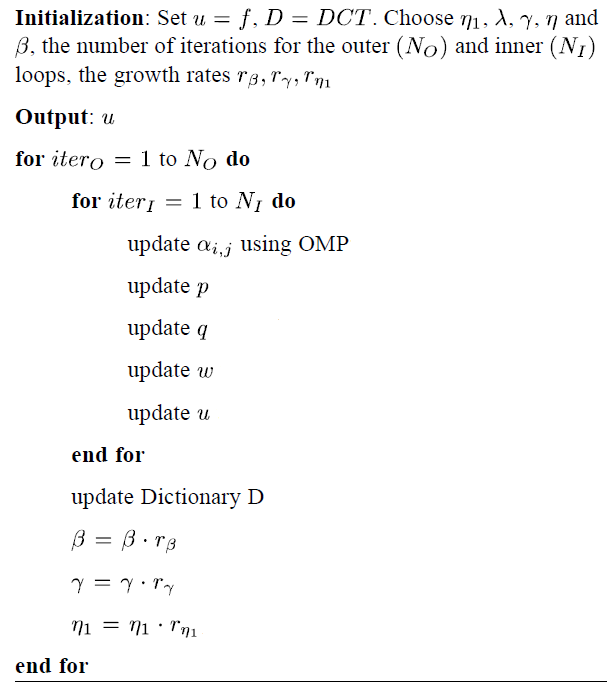
\includegraphics[scale=0.48]{algo.PNG}

\end{frame}

\section{Results}
\begin{frame}[t]{Experimental Results}{Benchmarks}
\begin{itemize}
    \item Comparisons made to the TV-Based algorithm (PIDSplit+) and the frame based algorithm (PIDAL-FA)
    %\item Images used are from MRI and Fluroescence Miscroscopy, followed by natural images
    \item Quality of restoration results compared quantitatively by using the PSNR: 
    \[
    PSNR = 20log_{10} \frac{Peak}{\frac{1}{mn} ||u^* - u ||_2}
    \]
    \item Stopping criterion:
    \[
    \frac{||u^{k+1} - u^k||_2}{||u^{k+1}||_2} < \epsilon
    \]
    
\end{itemize}
\end{frame}



\begin{frame}{Results}{Biomedical Images}
\begin{figure}
    \centering
    \includegraphics[scale=0.55]{Result_OriginalImages.PNG}
    %\caption{Caption}
    %\label{fig:my_label}
\end{figure}

\begin{figure}
    \centering
    \includegraphics[scale=0.55]{Result_Ankle.PNG}
    %\caption{Caption}
    %\label{fig:my_label}
\end{figure}

\end{frame}

\begin{frame}{Method Noise}

Evaluation metric that is adaptive to Poisson Noise. Uses the Anscombe transform. 

\[
A(u) - A(D_h u)
\]
Applying the Anscombe transform on both leads to a Gaussian approximation.
\end{frame}

\begin{frame}{Method Noise and Natural Images}

\begin{figure}
    \centering
    \includegraphics[scale=0.55]{Result_Brain1.PNG}
    %\caption{Caption}
    %\label{fig:my_label}
\end{figure}

\begin{figure}
    \centering
\includegraphics[scale=0.55]{Result_NaturalImages_Original.PNG}
    %\caption{Caption}
    %\label{fig:my_label}
\end{figure}
\end{frame}

\begin{frame}{Natural Images Results}
    \begin{figure}
        \centering
        \includegraphics[scale=0.5]{Result_NaturalImages.PNG}
        %\caption{Caption}
        %\label{fig:my_label}
    \end{figure}
\end{frame}

\begin{frame}{Tabular Results}{Natural Images}
    \begin{figure}
        \centering
        \includegraphics[scale=0.45]{Table_result.png}
        \caption{Natural Images}
        %\label{fig:my_label}
    \end{figure}
\end{frame}

\begin{frame}{Learned Dictionary}
\begin{figure}
    \centering
    \includegraphics[scale=0.5]{Dictionary_Medical}
    \caption{Learned Dictionary}
    \label{fig:my_label}
\end{figure}
    
\end{frame}

%\begin{frame}{Natural Images Result}
%    \begin{figure}
%        \centering
%        \includegraphics[scale=0.45]{Result_Sec2.PNG}
%        %\caption{Caption}
%        %\label{fig:my_label}
%    \end{figure}
%\end{frame}

%\begin{frame}{}
%   \begin{figure}
%        \centering
%       \includegraphics[scale=0.45]{Result_Sec3.PNG}
%        %\caption{Caption}
%        %\label{fig:my_label}
%    \end{figure}
%\end{frame}




\section{Discussion}
\begin{frame}[t]{Discussion}{Blind Deblurring}
\textbf{Blind deblurring}\\
\begin{itemize}
    \item We assume the blur kernel $H$ is known
    \item Not likely in real applications
    \item All existing methods used the Gaussian assumption
    \item Handles Poisson noise via a Variance Stabilization Transform
    \item Experiment includes images corrupted with a Gaussian blur and Poisson noise.
\end{itemize}
\end{frame}

\begin{frame}{Blind Deblurring}

\begin{figure}
    \centering
    \includegraphics[scale = 0.45]{Result_Sec2.PNG}
    \caption{}
\end{figure}
    
\end{frame}

\begin{frame}[t]{Discussion}{Multiplicative noise}
\textbf{Multiplicative noise}
\begin{itemize}
    \item Appears in laser imaging, ultrasound, synthetic aperture radar
    \item Can be modeled as 
    \[
        f = (Hu)M_n
    \]
    Where $M_n$ is a random variable with mean one
    \item The Data-Fidelity prior still appropriate if $M_n$ follows Gamma distribution
    \[
        P(x;\theta, L) = \frac{1}{\theta^L\Gamma(L)}x^{L-1}e^{-\frac{x}{\theta}} \quad \textrm{for} \quad x \geq 0
    \]
    Assume means equal to 1, so $L\theta=1$
\end{itemize}
\end{frame}

\begin{frame}[t]{Discussion}{Effect on parameters}
    \textbf{The Effect of the Parameters}
    \begin{figure}
        \centering
        \includegraphics[scale=0.33]{PSNR_VS_LAMBDA.PNG}
    \end{figure}
    \footnotesize{
        The $y$ axis is PSNR and $x$ axis is the $\lambda$ \\
        $\eta$ controls effect on TV, and TV also affect by ratio of $\eta$ and $\lambda$
    }
\end{frame}

\begin{frame}[t]{Discussion}{Effect on convergence}
    \textbf{The Effect of the convergence of the Algorithm}
    \begin{figure}
        \centering
        \includegraphics[scale=0.33]{ObjectiveFunc.PNG}
    \end{figure}
    \footnotesize{
        The $y$ axis is the error rate and $x$ axis is the iteration \\
        Gaussian blur and Poisson noise with peak at 600
    }
\end{frame}

\begin{frame}[t]{Discussion}{Computation time and improvements}
\textbf{Computation time and improvements}
\begin{itemize}
    \item Set $N_I=60$, $N_O=20$, $512\times 512$ image
    \item Takes 10 minutes
    \item Having to deal with $q \in \mathbb{R}^{mn} \times \mathbb{R}^{mn}$
    \item PIDSplit+ and PIDAL-FA take less than 1 minute
    \item Use faster computer!
    \item Parallel computing
    \item Early stop from the outer loop
\end{itemize}
\end{frame}

\section{Conclusion}
\begin{frame}[t]{Conclusion}
Conclusion

\begin{itemize}
    \item Generalized Blind Deblurring 
    \item Computation time 
    \item Non-Gaussian extensions
\end{itemize}
\end{frame}

\begin{frame}{}

\vspace{3cm}

Questions?
    
\end{frame}


\end{document}